\documentclass{book}
\usepackage{amsmath, amssymb}
\usepackage{ulem}
\usepackage{mathptmx}
\usepackage{ctex}
\usepackage{tcolorbox}
\usepackage{epigraph}
\usepackage{caption}
\usepackage{subcaption}
\usepackage{pdfpages}
\usepackage{graphicx}
\usepackage{multicol}
\setkeys{Gin}{width=0.75\textwidth}
\usepackage{listings}
\newtheorem{theorem}{Theorem}
\newtheorem{definition}{Definition}
\newtheorem{lemma}{Lemma}
\usepackage{tikz}
\usepackage{pifont}
\usepackage{threeparttable}
\usepackage{tabularx}
% \usepackage{algorithm}
\usepackage[lined,boxed,ruled]{algorithm2e}
\usepackage{bm}


% 在part页添加内容
\makeatletter
\let\old@endpart\@endpart
\renewcommand\@endpart[1][]{%
    \begin{quote}#1\end{quote}%
    \old@endpart}
\makeatother


\newcommand\tips[1]{\textcolor{green!50!black}{#1}}
\newcommand\notes[1]{\textcolor{blue!50!black}{#1}}
\newcommand\important[1]{\textcolor{red!90!black}{#1}}
\newcommand\warning[1]{\textcolor{orange!90!black}{#1}}

\newcommand\figures[2]{
    \begin{figure}
        \centering
        \includegraphics{../img/#1.png}
        \caption{#2}
        \label{#1}
    \end{figure}
}

\usepackage{enumitem}
% 去掉enumerate、itemize、description中的间隙
\setlist{noitemsep, topsep=0pt}

\tcbuselibrary{breakable}
\tcbset{breakable}
% \newtcblisting[auto counter, number within =chapter]{py}[1]{listing engine=minted,
% 	minted style=colorful,
% 	minted language=python,
% 	minted options={breaklines,autogobble,linenos,numbersep=3mm},
% 	colback=red!5!white,colframe=orange!50!blue,listing only, left=5mm,enhanced,
% 	title=Examples~\thetcbcounter~#1,
% 	breakable,
% 	enhanced
% 	%						 overlay={
% 	%						 	\begin{tcbclipinterior}
% 	%						 		\fill[red!30!white] (frame.south west)
% 	%						 		rectangle ([xshift=5mm]frame.north west);
% 	%							\end{tcbclipinterior}}
% }
\usepackage[
    top=1.23in,
    bottom=1in,
    right=1in,
    left=1in]
{geometry}

\usepackage{hyperref}
% 将引用的chapter改写为Chapter
\usepackage[english]{babel}
\addto\extrasenglish{
    \def\chapterautorefname{Chapter}
}
\addto\extrasenglish{
    \def\sectionautorefname{Section}
}
\usepackage{orcidlink}
\definecolor{SWJTU}{HTML}{025483}
% 全局取消段前缩进
% \setlength{\parindent}{0pt}
% \setlength{\parskip}{5pt}
\hypersetup{
    colorlinks=true,
    linkcolor=SWJTU,
    filecolor=SWJTU,
    urlcolor=SWJTU,
    citecolor=SWJTU,
}



\setkeys{Gin}{width=0.55\textwidth}
\begin{document}
\frontmatter
\begin{multicols}{2}
    \tableofcontents
\end{multicols}
\chapter*{前言}
\section{一些私人理解}
很多 pattern 分析的心理都是空和多,但是下跌中,如果只是有本持有的多方卖出,他们并不一定需要回补,那么看涨情绪在不能做空的市场中应该要稍弱。
\mainmatter
% \chapter{金融数据及其特征}
\section{资产收益率}
大多数金融研究都是针对资产收益率,而不是资产价格. Campbell 等(1997)给出了使用资产收益率的两个主要原因. 首先,对于一个普通的投资者来说,资产收益率代表一个完全的、尺度自由的投资机会的总结和概括. 其次,资产收益率序列比价格序列更容易处理,前者有更好的统计特性. 然而,资产收益率有多种不同的定义.
\subsection*{单期简单收益率}
假设投资者在一个周期内拥有某种资产,从第 $t-1$ 天到第 $t$ 天,其简单毛收益率为:
$$1+R_t=\frac{P_t}{P_{t-1}} ~\text{or} ~P_t=P_{t-1}(1+R_t)$$

相对应的单期简单净收益率 (simple net return)或简单收益率(simple return)为:
\begin{equation}
    R_t=\frac{P_t}{P_{t-1}}-1=\frac{P_t-P_{t-1}}{P_{t-1}}
\end{equation}

\subsection*{多期简单收益率}
假设从第 $t-k$ 天到第 $t$ 天,这 $k$ 个周期内持有某种资产,则 $k$ 期简单毛收益率为:
\begin{equation}
    \begin{aligned}
        1+R_t[k] & =\frac{P_t}{P_{t-1}}=\frac{P_t}{P_{t-1}}\times\frac{P_{t-1}}{P_{t-2}}\times\cdots\times\frac{P_{t-k+1}}{P_{t-k}} \\
                 & =(1+R_t)(1+R_{t-1})\cdots(1+R_{t-k+1})                                                                           \\
                 & =\prod_{j=0}^{k-1}(1+R_{t-j})
    \end{aligned}
\end{equation}
这样,$k$ 期简单毛收益率是其包含的这 $k$ 个单期简单毛收益率的乘积,称为复合收益率 (compound return). $k$ 期简单净收益率为 $R_t[k]=(P_t -P_{t-k})/P_{t-k}$.

在实际中,确切的时间区间对讨论和比较收益率是非常重要的(例如月收益率还是年收益率). 若时间区间没有给出,这里隐含的假定时间区间为一年. 如果持有资产的期限为 $k$ 年,则(平均)年度化收益率定义为
$$\text{年化}R_t[k]=\left[\prod_{j=0}^{k-1}(1+R_{t-j})\right]^{1/k}-1$$

这是由它所包含的 $k$ 个单期简单毛收益率几何平均得到的,可用下式计算:
$$\text{年化}R_t[k]=\exp\left[\frac{1}{k}\sum_{j=0}^{k-1}(1+R_{t-j})\right]-1$$

因为算术平均值比几何平均值计算起来容易,并且单期收益率一般很小,所以我们可用一阶泰勒(Taylor)展开来近似表示年度化的收益率,则有
\begin{equation}
    \label{eq1-3}
    \text{年化}R_t[k]\approx\frac{1}{k}\sum_{j=0}^{k-1}R_{t-j}
\end{equation}
然而,在有些应用中,\autoref{eq1-3} 的近似精确度可能不够.
% \part{基本知识}
% % \chapter{其他买入看涨期权的策略}
我们将讨论另外两种买入看涨期权的策略。这两种策略都涉及卖空标的股票和买入看涨期权。当标的股票有场内看跌期权交易的时候,这些策略就没有使用看跌期权那么好。不过,这里的概念相当重要,并且当市场中看涨期权非常活跃而看跌期权不活跃时,这些策略就会更有活力。这些策略一般被称为“合成”(synthetic)策略。
\section{保护性卖空(合成看跌期权)}
在卖空标的股票的同时买入看涨期权,是将卖空的风险限制在一定数额里的一种手段。从理论上来说,卖空的风险是无限的,因此许多投资者在卖空时都会有所顾虑。对这些卖空股票的投资者来说,股票价格的上涨会让他们心绪不安。投资者有可能会由于情绪的缘故而被迫作出也许是不正确的决定——回补卖空头寸,以减低心理压力。如果在卖空股票的同时持有看涨期权,投资者就可以把亏损限制在一个固定的、通常是相当小的数额内。

当投资者买入看涨期权来保护卖空头寸时,有一个简单的公式可以计算最大风险金额:
\begin{equation}
    \text{风险}=\text{买入的看涨期权的行权价}+\text{看涨期权价格}–\text{股票价格}
\end{equation}

无论是上涨还是下跌,卖空者的风险都会因标的股票发放股息而略有增长,因为他必须为卖空的股票支付股息。

一般而言,最好是买入平值或略微虚值的看涨期权来对卖空头寸进行保护。买入深度虚值看涨期权在保护方面起不到什么作用,除非股价急剧上涨,否则它对风险没有什么改善。正常情况下,投资者会在卖空头寸对其产生严重不利后果之前就回补。因此,花钱买入这样一个深度虚值看涨期权是一种浪费。不过,如果投资者想要他的卖空头寸有足够的“活动”空间,并且非常肯定他对这个股票极度看空的看法是正确的,那么他可以买入相当深度的虚值看涨期权来作为灾难保护,以防股票价格突然向上爆发(例如,标的股票突然收到收购要约)。

\begin{figure}
    \centering
    \begin{tikzpicture}[scale=.4,shift={(35,0)}]
        \draw[->] (35, 0) -- (47, 0) node[anchor=north] {\small{到期时标的资产价格}};
        \draw[->] (35, -6) -- (35, 6) node[anchor=east] {\small{到期时盈亏}};
        \draw[thick] (35,2)--(37,0)node[anchor=north east]{0}--(40,-3)--(45, -3);
        \draw[dashed] (37,3)--(40,0)node[anchor=north east]{40}--(45, -5);
        \draw[dashed] (40, 0)--(40, -3)node[anchor=north east]{-3};
    \end{tikzpicture}
    \begin{tikzpicture}[scale=.4,shift={(35,0)}]
        \draw[->] (35, 0) -- (47, 0) node[anchor=south] {\small{到期时标的资产价格}};
        \draw[->] (35, -6) -- (35, 6) node[anchor=east] {\small{到期时盈亏}};
        \draw[thick] (36,3.5)--(39.5,0)node[anchor=north east]{0}--(45, -5.5)--(46,-5.5);
        \draw[dashed] (37,3)--(40,0)node[anchor=south west]{40}--(46, -6);
        \draw[dashed] (45, 0)--(45, -5.5)node[anchor=north east]{-5.5};
        \fill (45, 0) circle (3pt);
    \end{tikzpicture}
    \caption{卖空者愿意承担的风险可能不同,他也许想买入1手虚值看涨期权作为保护,而不是上面示例中的平值看涨期权。如果买入的是虚值看涨期权,保护成本就会低一些,卖空者所放弃的潜在盈利也少一些。但是他的风险就会大一些,因为只有在股票上涨到行权价之上的时候,这个看涨期权才具有保护功能。}
\end{figure}
\section{保证金要求}
根据最新的保证金规则,如果股票空头头寸有看涨期权多头保护,投资者在保证金要求方面就会有相当的优待。实际所需的保证金为下列两项的较小值:第一,看涨期权行权价的 10\% 加上虚值部分的金额;第二,卖空股票现有市场价值的 30\%。这个头寸会被逐日盯市,如果股票价格低于行权价,大部分经纪商会要求该卖空头寸按“正常”比率缴纳保证金。
\section{组合保证金}
一般而言,组合保证金要求是基于风险的,很难手工计算出来。
\section{后续行动}
保护性卖空者在这个策略中需要采用的后续行动基本上就是平仓。如果标的股票先迅速下跌,然后看上去会反弹,那投资者应该回补股票,而不是卖出看涨期权。这样做的话,如果股票反弹到最初的行权价之上,投资者还能从看涨期权中获利。如果标的股票价格上涨,那就不应该采取相似的、只卖出盈利头寸(看涨期权)的方法。也就是说,如果 XYZ 从 40 涨到了 50,而 7 月 40 看涨期权价格也从 3 涨到了 10,那就不应只卖出看涨期权获得 7 点盈利,并继续持有股票以希望其会下跌。理由是,当看涨期权为实值时,如果解除保护,这个投资者就会面临高度的风险。如果股票价格下跌,那么提走盈利就不是问题,这甚至是他所期望的。因为如果股票继续下跌,就没有或者只有很小的额外风险。但当股票上涨时,情况就不同了。在这种情况下,如果卖空者卖掉他的看涨期权拿走盈利,而股票随后继续上涨的话,就会产生大笔的亏损。

如果看涨期权是持平(at parity)或接近持平的,或者是实值的,那么通过行权而把头寸平仓,就常常是可取的做法。在大多数策略里,由于股票手续费比期权手续费高出许多,将看涨期权行权对期权持有者来说没有什么好处。但在保护性卖空的策略里,卖空者最终总是要回补他卖空的股票,因而总会有股票手续费。因此,行权并按行权价(也就是较低的价格)买入股票,或许还能因此少支付些手续费,这也许会给他带来好处。
\section{合成跨式价差(反向对冲)}
在这种策略里,投资者买入的看涨期权所对应的股数要多于其卖空的股数。如果在期权的存续期内标的股票上涨或下跌的幅度足够大,这个策略家就可以盈利。这个策略一般被称作反向对冲(reverse hedge)或合成跨式价差(synthetic straddle)。如果该股票有场内看跌期权交易,那这个策略就过时了,直接买入跨式价差(1 手看涨期权和 1 手看跌期权)所产生的结果会更好。因此,这个反向对冲策略又被称为“合成跨式价差”。

如果股票在任何方向上有足够幅度的运动,显然都可以得到盈利。事实上,投资者可以准确地判断出,如果要盈利,在到期时股票必须达到怎么样的价格。这些盈亏平衡点很容易计算出来。首先计算出最大风险,然后再确定盈亏平衡点。
\begin{equation}
    \begin{aligned}
        \text{最大风险}    & =\text{行权价}+2\times \text{涨期权价格}-\text{股票价格} \\
        \text{上行盈亏平衡点} & =\text{行权价}+\text{最大风险}                      \\
        \text{下行盈亏平衡点} & =\text{行权价}-\text{最大风险}                      \\
    \end{aligned}
\end{equation}

在到期之前,即使股价离行权价很近也有可能盈利,因为买入的看涨期权还剩有时间价值。

一般而言,进行合成跨式价差交易的股票的波动率应该较大。尽管这种股票的期权权利金会比较高,但当价格呈直线运动时,股票价格的变化幅度仍会大于这些权利金。使用波动率较大的股票的另一个好处是,一般它们很少或者没有股息。这是合成跨式价差所期望的,卖空者也就不必付或者只需付很少的股息。

在建立头寸时,标的股票的技术形态也会有帮助。交易者一般希望在策略亏损的区域内不存在技术性的支撑位和压力(resistance)位。在这样的形态里,股票可以上下快速运动。交易者有时也可以交易宽幅震荡的股票,它们的股价不断地在震荡区域的这一端摆动到另一端。如果反向对冲的亏损区域刚好位于该震荡区间之内,那这个头寸也会有吸引力。
\section{后续行动}
因为反向对冲内在的有限亏损特征,所以没有必要采取任何后续行动来限制亏损。投资者可以相当容易地建立头寸,在到期日前也不必采取任何后续行动。在这个策略里,这经常就是最好的后续行动。

另外,还有一种后续行动可以运用,尽管这种行动有一定的不利之处。它有时被称为针对跨式价差的交易(trading against the straddle)。当股价在任何一个方向运动得足够远的时候,就从这一侧提取盈利。然后等股价摆回到另一个方向时,就再从另一侧提取盈利。
\section{改变看涨期权多头和股票空头之间的比率}
资者不一定非要刚好买入 2 手看涨期权来对应 100 股股票空头。他可以就 100 股股票空头买入 3 或 4 手看涨期权,以建立一个更为看多的头寸。

不管比率是多少,都可以用一个公式来计算最大风险和盈亏平衡点。
\begin{equation}
    \begin{aligned}
        \text{最大风险}    & =(\text{行权价}-\text{股票价格})\times \text{卖空的股票手数}+\text{买入的看涨期权手数}\times \text{看涨期权价格} \\
        \text{上行盈亏平衡点} & =\text{行权价}+\frac{\text{最大风险}}{\text{买入的看涨期权手数}-\text{卖空的股票手数}}                     \\
        \text{下行盈亏平衡点} & =\text{行权价}-\frac{\text{最大风险}}{\text{卖空的股票手数}}                                      \\
    \end{aligned}
\end{equation}

这个策略可以使用的最后一种调整方法,就是在卖空 100 股股票的同时,买入 2 手行权价不同的看涨期权。于这个策略涉及两个行权价,因此被称为“合成宽跨式”(synthetic strangle),即由两个行权价不同的看涨期权或看跌期权构成的普通跨式。
\section{总结}
如果标的股票有场内看跌期权,这一章所描述的策略一般就没有用处。但是,如果没有看跌期权存在,或者看跌期权很不活跃,而策略家认为在看涨期权的存续期内股票会在某一方向上有相对较大的运动,他就应当考虑使用某种形式的合成跨式策略,也就是卖空一定数量的股票,同时买入对应更多股票数量的看涨期权。如果他所希望的运动确实出现了,就会产生可观的盈利。无论是哪种情况,亏损都被限制在某个固定的金额之内,一般是初始头寸的 20\%-30\%。虽然可以采取一些后续行动来锁住小额盈利和从股票的反向运动中获利,但更明智的做法是继续持有头寸,以便获得更大的盈利。这个策略一般使用 2:1 的比率(买入 2 手看涨期权,卖空 100 股股票),但如果投资者想要更为看多或者看空,可以调整这个比率。如果初始股票价格在两个行权价之间,可以通过在卖空股票的同时分别买入次高行权价和次低行权价的看涨期权,来建立一个中性的盈利区域。
% \chapter{酒田战法和其他蜡烛图组合}
\section{酒田战法}
\subsection{三山形态}
三山形态构成了市场的一个大型顶部,与西方技术分析中的“三重顶”形态比较类似,在三重顶形态中,价格上升和下跌各三次,形成了市场的顶部。三尊顶形态(san-son)与西方的头肩形顶部形态也类似。三尊顶形态有点儿像佛教中佛像的陈列,大殿里供奉的佛像通常有三尊,其中中间摆放的是一尊最大的,两边分别是小一点的佛像(见 \autoref{fig5-1a})。三山形态包含了西方技术分析中的“三重顶”形态,在这一形态中,价格三次向上测试,但随后都出现了一定幅度的调整,在三重顶形态中,三个顶部的高度是相同的,或者大致接近(见 \autoref{fig5-1b})。
\figures{fig5-1a}{}
\figures{fig5-1b}{}

\subsection{三川形态}
三川形态和三山形态正好相反。它同传统的三重底形态和头肩底形态类似。三川形态由三根位于市场底部的看涨蜡烛线组合而成,用于预测市场的转折点,这些 K 线组合包括启明星、白三兵等,在一些介绍酒田战法的日文著作中,也将启明星形态称作三川启明星形态 \autoref{fig5-2a}。

\figures{fig5-2a}{}
\subsection{三空形态}
在三空形态中(\autoref{fig5-3}),价格的跳空缺口意味着投资者进入和退出市场的时机。以向上跳空形态为例,市场出现底部后,当它再次上升时,投资者应该在出现第三个跳空缺口后做空。第一个向上跳空缺口意味着新入场的买方力量强大,第二个缺口代表继续有买方入场以及部分有经验的空头平仓,第三个跳空缺口是由犹豫的空头平仓和如梦初醒的多头买进造成的。酒田战法建议在第三个向上跳空的缺口后做空,因为买盘卖盘出现分歧以及随后市场出现超买的可能性越来越大。相反,在下降趋势中出现第三个向下跳空缺口后,投资者应该做多。在日语中,跳空缺口的弥补又被称为“anaume”,跳空缺口又被称为窗口(mado)。

\figures{fig5-3}{}
\subsection{三兵形态}
三兵形态指的是“向同一个方向站立的三名士兵”。白三兵是一个典型的看涨信号,表明市场正处于稳定的上升态势中,这种稳健的价格走势说明市场将进一步大幅走高。另外,酒田战法还给出了三兵形态的衰退形态,这些形态表明上升趋势的力度逐渐减弱,也就是通常所说的“上涨乏力”。三兵形态包含几种衰退形态,第一种衰退形态是“前进受阻形态”,该形态虽然跟白三兵形态比较类似,不同之处在于,该形态在第二天和第三天录得的 K 线都带有很长的上影线。第二个衰退形态则是“停滞形态”,在该形态中,同样也是第二天的 K 线带有很长的上影线,而第三天则是出现纺锤线,或者是十字星,这表明市场拐点的临近。
% \chapter{卖出看涨期权比率}
\section{卖出看涨期权比率}
简单地说,卖出看涨期权比率(ratio call writing)是这样一种策略,投资者持有一定数量的标的股票,同时他卖出了更多股数的看涨期权。因此,卖出的看涨期权所对应的股数与已持有的股数之间就有了一个比率。最常见的比率是 2:1,在这种比率上,投资者持有 100 股标的股票,同时卖出 2 手看涨期权。请注意,这类头寸涉及卖出一定数量的裸期权以及一定数量的备兑期权。由此而产生的头寸,既有卖出备兑看涨期权时的下行风险,又有裸卖出时的无限上行风险。如果标的股票价格在期权存续期内保持相对无变化,卖出看涨期权比率的盈利会比只卖出备兑看涨期权和只卖出裸看涨期权都要大得多。不过与卖出备兑看涨期权和裸看涨期权不一样,卖出看涨期权比率在两个方向上都面临风险。

一般而言,某个投资者在建立卖出看涨期权比率头寸的时候,他应当对标的股票的前景保持中立。这就是说,他卖出的是行权价最接近当前股票价格的看涨期权。
\begin{figure}
    \centering
    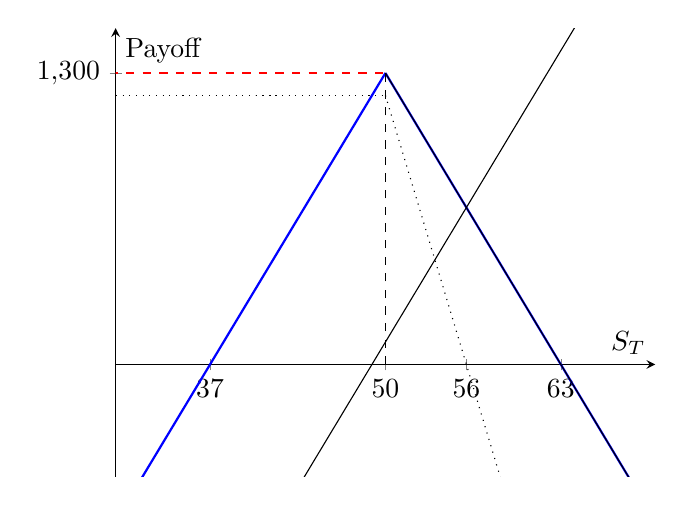
\begin{tikzpicture}
        \begin{axis}[
                axis lines=middle,
                xlabel={$S_T$},
                ylabel={Payoff},
                xmin=30, xmax=70,   % 调整x轴的范围
                ymin=-500, ymax=1500, % 调整y轴的范围
                xtick={37,50,56,63},
                ytick={1300},
                domain=0:100, % 调整绘制曲线的 x 轴范围
                samples=100,
            ]
            % 设置期权参数
            \pgfmathsetmacro\K{50} % 执行价格
            \pgfmathsetmacro\multiplier{100} % 合约乘数

            % 画看涨期权到期收益线
            \addplot[thick,blue,domain=0:50] {(x-37) * \multiplier};
            \addplot[thick,blue,domain=50:100] {(63-x) * \multiplier};
            \addplot[domain=50:100] {(63-x) * \multiplier};
            \addplot[] {(x-49) * \multiplier};
            \addplot[domain=0:\K,dotted] {2 * 6 * \multiplier};
            \addplot[domain=\K:100,dotted] {2 * (56-x) * \multiplier};

            % 在执行价格标注
            \draw[thick,red,dashed] (axis cs:0,1300) -- (axis cs:\K,1300);
            \draw[dashed] (axis cs:\K,0) -- (axis cs:\K,1300);
        \end{axis}
    \end{tikzpicture}
    \caption{期权到期收益图:通过按 49 买入 100 股 XYZ 股票,同时按每手 6 点卖出 2 手 XYZ 10 月 50 看涨期权来建立一个卖出看涨期权比率头寸。}
\end{figure}
% % \chapter{持续形态}
所谓的持续性形态,意味着形态完成后,市场仍将恢复先前的趋势。举例来说,如果在上涨行情之后出现了持续形态,那么我们预期上涨行情仍在发挥作用。(当然,这一点并不排除在持续形态出现后先发生调整行情,调整之后再恢复原先的涨势。)

将要讨论的持续形态有窗口(以及含有窗口的一些蜡烛图形态)、上升三法、下降三法、分手线,以及白三兵形态。

\section{窗口}
日本技术分析师一般把西方所说的价格跳空称为窗口。按照西方的表达方式,我们说“回填跳空”;在日本,人们则说“关上窗口”。这一部分,我们先来阐述窗口的基本概念,然后还要探讨包含窗口(价格跳空)的其他一些形态。

窗口有两种类别,一种是看涨的,一种是看跌的。\textbf{向上的窗口}(如 \autoref{fig7-1} 所示)是看涨信号。在前一个时段最高点(也就是其上影线的顶端)与本时段最低点(也就是其下影线的底端)之间,存在价格上的真空地带。

\figures{fig7-1}{向上的窗口}

\autoref{fig7-2} 展示了一例\textbf{向下的窗口}。它是看跌信号。在前一个时段最低点与本时段最高点之间,存在价格缺口。

\figures{fig7-2}{向下的窗口}

根据日本技术分析师的观点,市场参与者应当顺着窗口形成的方向建立头寸。这是因为窗口属于持续性质的技术信号。因此,如果出现了向上的窗口,我们就应该利用市场回落的机会逢低买进;如果出现了向下的窗口,就应该利用市场反弹的机会逢高卖出。

日本人还认为:“调整行情于窗口处终结。”这意味着窗口可能转化为支撑区域或阻挡区域。于是,如果出现了向上的窗口,则在今后市场向下回撤时,这个窗口将形成支撑区域(我们马上会看到,这是指窗口的全部空间)。如果市场在向下回撤时收市价达到了窗口下边缘之下的水平,那么,先前的上升趋势就不复成立了。请注意,在 \autoref{fig7-1} 中,市场在日内一度下跌到窗口下边缘之下,但是因为不是收市价低于该区域,所以向上的窗口所形成的支撑区域保持完好。

同样,如果出现了一个向下的窗口,则意味着市场还将进一步下降。此后形成的任何价格向上反弹,都会在这个窗口处遭遇阻挡(指窗口的全部空间)。如果多方拥有足够的推动力,将收市价推升到向下的窗口之上,那么,下降趋势就完结了。

在西方,一般认为价格跳空总要被回填。我不知道这一点是不是正确的,不过如果采用蜡烛图技术的概念“调整行情于窗口处终结”,那么当行情试图回填价格跳空时,便可以考虑买进(在向上的窗口处)或卖出(在向下的窗口处)。

对窗口最常发生的误解是,有些人误以为如果两根蜡烛线的实体之间不相接触,那么这两根蜡烛线便组成了一个窗口。正如 \autoref{fig7-1} 和 \autoref{fig7-2} 所示,组成窗口的蜡烛线必须是其影线之间互不重叠。无论两根蜡烛线实体之间的“缺口”有多大,除非在它们的影线之间存在缺口,否则不构成窗口。

如 \autoref{fig7-3} 所示,在 7 月 22 日的最高点和次日的最低点之间仅有 4 美分的空白,这是一个小型向上的窗口。无论向上的窗口多么小,它都应当构成潜在的支撑区域。对于向下的窗口,同样也应当构成阻挡区域。窗口不在乎尺寸大小。在 \autoref{fig7-3} 中,向上的窗口形成了支撑区域,之后当行情回落到接近其支撑区域时,留下了一些长长的下影线,突出显示此处需求强大。正如本图所示,虽然向上的窗口构成潜在的支撑区域,但是市场并不需要精确地回落到窗口所在的支撑区域之后才能向上反弹,有时甚至连接近它都谈不上。因此,在市场朝着向上的窗口回落的过程中,如果您积极看好,那么甚至当市场接近该窗口的上缘时,便可以考虑买进了,无须等到行情进入该窗口之内。如何运用窗口,取决于您的交易风格和交易的迫切程度。应当事先设置止损措施(做好思想准备或者其他措施),以防止行情收市于向上的窗口的下缘之下。

\figures{fig7-3}{轻质原油——日蜡烛线图(向上的窗口)}
在 \autoref{fig7-4} 中,在 20.50 美元和 22.50 美元之间存在一个幅度非常大的窗口。这么一来,它构成了一个幅度达 2 美元的支撑区域(从窗口的顶部 22.50 美元到窗口的底部 20.50 美元)。

在窗口幅度相对较大的情况下,请记住,向上的窗口的关键支撑水平位于窗口的底部(相应地,向下的窗口的关键阻挡水平位于窗口的顶部)。因此,在向上的窗口中,其支撑作用的“最后一口气”就是图上用虚线标注的窗口的底部(即价格跳空的下边缘)。

下面再看看另外两个向上的窗口,图上分别用 1 和 2 来做了标记。窗口 1 的支撑作用在其出现后三周之内一直维持良好,直到 4 月 6 日的蜡烛线才向下突破了该支撑水平。窗口 2 的支撑作用在其出现之后的第二天便被向下突破了。在窗口 2 被向下突破后,窗口 1 发挥了支撑作用。这就是我运用窗口的具体做法。举例来说,如果某个窗口的支撑被突破,那就在被突破的窗口下方寻找另一个窗口,以后者作为下一个支撑区域。在本图中,一旦窗口 2 被向下突破,下一个支撑位置便是窗口 1。

\figures{fig7-4}{网威公司(Novell)——日蜡烛线图(向上的窗口)}

单一的蜡烛图信号是否值得采信,必须首先从其所处的总体技术背景来考虑。\autoref{fig7-5} 的实例充分显示了这一点的重要性。3 月 1 日的第一根蜡烛线是看涨的锤子线。但是更重要的是,看看这根锤子线是如何形成的——一个向下的窗口。一方面,锤子线本身立即构成了支撑水平;另一方面,切不可忘记,因为这个向下的窗口,窗口的整个空间现在都成为阻挡区域。果然,从锤子线开始的反弹行情到向下的窗口顶边时渐渐熄火了。
\figures{fig7-5}{亚马逊——5 分钟蜡烛线图(向下的窗口)}

传统的日本技术分析理论认为,在三个向上的或向下的窗口之后,很可能市场已经处在过度超买状态,上升行情难以为继(在三个向上的窗口的情形下),或者处在过度超卖状态,下降行情无力维持(在三个向下的窗口的情形下)。

窗口的地位如此显要,无论已经出现了多少个窗口,当前的趋势都不受影响,直到最后的窗口被关闭为止。在上升行情中,可以有任意数目的向上的窗口。只要市场没有以收市价向下突破最高的那个向上的窗口,则趋势依然维持向上。

在 \autoref{fig7-8} 中,展示了这样的一个实例。8 月中旬于 B 处形成了一个看涨的吞没形态,由此开始形成了一轮上冲行情。最终,这轮行情总共打开了六个向上的窗口。10 月  5日和 6 日组成了一个孕线形态,这是我们得到的最早的线索,表明债券市场喘不过气来了。但是,要等到收市价向下突破了第六个向上的窗口之后,这轮上冲行情才终结。后来的结果表明,债券期货行情此处的向下反转形成了一个主要的历史高点,之后市场多年保持下滑态势。

\figures{fig7-8}{债券期货——日蜡烛线图(向上的窗口)}
\section{向上跳空和向下跳空并列阴阳线形态}
\textbf{并列阴阳线形态}是由具备特定形态的两根蜡烛线组成的,两者一起向上跳空或向下跳空。\autoref{fig7-10} 为向上跳空并列阴阳线形态,其中一根白色蜡烛线和一根黑色蜡烛线共同形成了一个向上的窗口。这根黑色蜡烛线的开市价位于前一个白色实体之内,收市价位于前一个白色实体之下。在这样的情况下,这根黑色蜡烛线的收市价,就构成了买卖双方争夺的要点。如果市场以收市价向下突破到该窗口之下,那么这个向上跳空并列阴阳线形态的看涨意义就不再成立了。在向下跳空并列阴阳线形态中,基本概念与上述形态是相同的,只不过方向相反。一根黑色蜡烛线和一根白色蜡烛线共同打开了一个向下的窗口。在向上跳空和向下跳空并列阴阳线形态中,两根蜡烛线的实体的大小应当不相上下。两种跳空并列阴阳线形态都很少见。

\figures{fig7-10}{向上跳空并列阴阳线形态}

在 \autoref{fig7-12} 中,9 月底出现了一个小型向上的窗口。在向上的窗口之后有两根蜡烛线,组成了向上跳空并列阴阳线形态。之所以称之为并列阴阳线形态,是因为在向上的窗口之后,先是一根白色蜡烛线,然后是一根黑色蜡烛线。然而上面刚刚指出,依我看来,在向上的窗口之后,到底那两根蜡烛线是什么样子并不要紧。\important{主要的考虑是把向上的窗口视为支撑区域,并根据收市价来判断其守与破}。正如图上虚线所示,根据收市价来判断,该支撑区域无论如何总算维护住了。后来,10 月底出现了一根看涨的捉腰带线,并且它包裹了之前的三根黑色实体,从而为该窗口的支撑作用给出了最终的验证信号。

\figures{fig7-12}{铂金——周蜡烛线图(向上跳空并列阴阳线)}
\subsection{高价位和低价位跳空突破形态\label{subsection7-2-1}}
在上升趋势中,当市场经历了一轮急剧的上涨后,在正常情况下都需要一个调整消化的过程。有时,这个整理过程是通过一系列小实体来完成的。如果在一根坚挺的蜡烛线之后,出现了一群小实体的蜡烛线,则表明市场已经变得犹豫不决了。虽然这群小实体表示行情趋势已经从向上转为中性,但是它们的出现在某种意义上是健康的,因为通过踩水的过程,缓解了市场所处的超买状态。一旦后来某一天的行情从这群小实体处打开了一个向上的窗口,就是看涨的信号。这就是一个\textbf{高价位跳空突破形态}(如 \autoref{fig7-13} 所示)。之所以这样称呼这类形态,是因为在这类形态中,市场先是在最近形成的高价位上徘徊,后来才下定决心向上跳空。
\figures{fig7-13}{高价位跳空突破形态}

可想而知,\textbf{低价位跳空突破形态}正是高价位跳空突破形态的反面角色,两者对等而意义相反。低价位跳空突破形态是一个向下的窗口,是从一个低价位的横向整理区间向下打开的。这个\textbf{横向整理区间}(一系列较小的实体)发生在一轮急剧下跌之后,曾经使市场稳定了下来。当初,从这群小实体蜡烛线的外观看来,似乎市场正在构筑一个底部。但是后来,市场以窗口的形式从这个密集区向下突破,打破了这种看涨的期望。

在 \autoref{fig7-15} 中,7 月 31 日是一根锤子线,结果成了之后上涨行情的低点,在这轮上涨中,8 月初曾经形成一个向上的窗口。在 8 月 7日所在的一周里,出现了一根长黑色实体,组成了乌云盖顶形态,在这轮上涨行情的前方添加了一块临时的挡板。

在 8 月 21 日所在的一周里,先是一根长长的白色蜡烛线,后面跟着一系列小实体,显示该股票行情已经进入调整阶段。8 月 28 日打开了一个小型向上的窗口,完成了一个高价位跳空突破形态,证明多头完全控制了市场。

\notes{在本形态中,或者在任何高价位跳空突破形态中,一旦市场收市于其中向上的窗口之下,则消除了形态的看涨意义。}对低价位跳空突破形态来说,道理相同而方向相反。
\figures{fig7-15}{康宁公司——日蜡烛线图(高价位跳空突破形态)}

在 \autoref{fig7-17} 中,4 月初的孕线形态有助于终结当时的上涨行情。从本形态开始市场下降并逐步加速,特别是 4 月 15 日的超长黑色实体加剧了下跌的进程。之后的两个时段都是纺锤线,有线索显示股票正在努力稳住。然而,4 月 17 日收市价再创新低,下一日又完成了一个低价位跳空突破形态,表明空头重新夺得全部控制权。

请观察 5 月初的小型窗口是如何转化为阻挡区域的。该阻挡区域很重要,值得牢记于心,因为在 1 处有一根锤子线,在 2 处又有一个看涨吞没形态,都是底部信号。但是在这两个看涨信号出现时,交易者对买进应当保持谨慎态度,因为根据该窗口的阻挡作用,潜在的利润空间有限。
\figures{fig7-17}{糖——日蜡烛线图(低价位跳空突破形态)}
\subsection{跳空并列白色蜡烛线形态}
在上涨行情中,先出现了一根向上跳空的白色蜡烛线,随后又是一根白色蜡烛线,并且后面这根线与前一根线大小相当,两者的开市价也差不多处在同样的水平上,这样就形成了一种看涨的持续形态。这种双蜡烛线形态称为\textbf{向上跳空并列白色蜡烛线形态}(或者称为\textbf{向上跳空并列阳线形态},如 \autoref{fig7-18} 所示)。

\warning{上面介绍的这种并列白色蜡烛线形态是很少见的}。不过,更少见的还有向下跳空的两根并列白色蜡烛线。这类形态称为向下跳空并列白色蜡烛线形态。在下跌行情中,尽管它们都是白色蜡烛线,因为之前向下的窗口,依然把它们归结为看跌信号。这是因为这两根白色蜡烛线被看作空头平仓的过程。一旦空头平仓的过程完成了,价格就要进一步下跌。这类向下跳空并列白色蜡烛线形态之所以特别罕见,其原因不难理解。在市场下降趋势中,当出现向下跳空时,如果形成跳空的蜡烛线是一根黑色蜡烛线,那么当然比一根白色蜡烛线自然得多。

\figures{fig7-18}{上升趋势中的向上跳空并列白色蜡烛线形态}

虽然下面也为这些形态提供了实例,但是形成跳空并列白色蜡烛线形态的蜡烛线的具体情况并不重要,无须死记硬背。重要的是形态中所包含的向上或向下的窗口。正如在 \autoref{subsection7-2-1} \nameref{subsection7-2-1} 讨论的那样,\tips{这两根蜡烛线的样式并没有多少影响,无论窗口之后的两根蜡烛线都是白色的(在跳空并列白色蜡烛线形态下),还是一根白色一根黑色的(在跳空并列阴阳线形态下)。唯有窗口本身提供了趋势信息,以及支撑区域或阻挡区域。}

\textbf{窗口,才是关键因素}。不论向上的窗口还是向下的窗口,窗口之后的两根蜡烛线的具体组合与颜色配合无关宏旨。向下的窗口推动趋势向下,向上的窗口推动趋势向上,并且窗口分别构成阻挡或支撑区域。
% \chapter{动态对冲}
\section{}
\subsection{}

\begin{figure}
    \centering
    \begin{subfigure}{0.45\textwidth}
        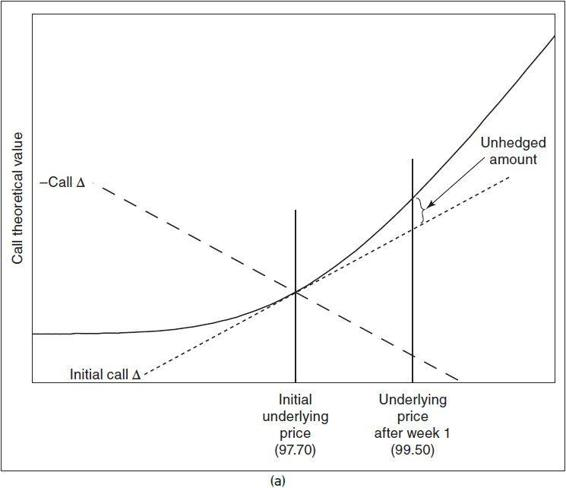
\includegraphics[width=\textwidth]{../img/fig8-3a.png}
        \label{fig8-3a}
    \end{subfigure}
    \hfill
    \begin{subfigure}{0.45\textwidth}
        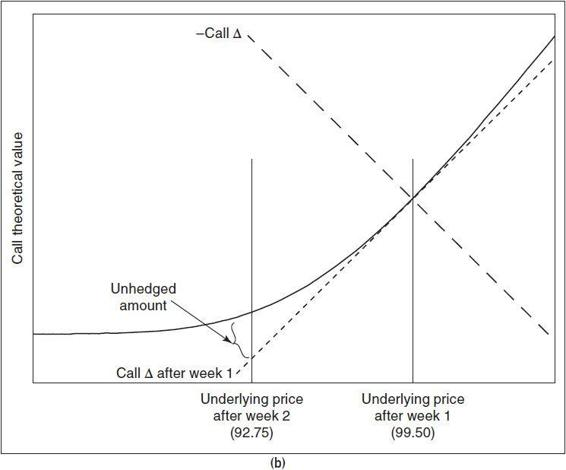
\includegraphics[width=\textwidth]{../img/fig8-3b.png}
        \label{fig8-3b}
    \end{subfigure}
    \caption{我们确定了标的物价格为 97.70 时的期权初始 delta(虚线),然后在标的合约中建立了一个 delta 相反的仓位(虚线)。当标的价格发生很小的变动时,一个仓位的利润可以抵消另一个仓位的损失。由于期权的曲率(其 gamma),当标的价格在任一方向上的变化变大时,这两个仓位之间就会出现不匹配。当标的价格下跌时,期权仓位贬值的速度开始下降;当标的价格上涨时,期权仓位升值的速度开始上升。在 (a) 中,我们可以看到标的价格为 99.50 时的这种不匹配或未对冲金额。当标的价格为 99.50 时,我们通过调整头寸以返回 delta 中性来捕捉这种错配的价值。这如 (b) 所示。我们重新计算了新标的价格下的 delta,并在标的合约中建立了新的对立头寸。当标的价格跌至 92.75 时,错配再次等于未对冲的金额。}
    \label{fig8-3}
\end{figure}

通过重新对冲头寸,我们能够获得一系列利润,这些利润源于期权不断变化的 delta 与标的合约固定 delta 之间的不匹配。当然,在时间流逝的同时,还有利息的考虑。但期权的大部分价值是由重新对冲过程中赚取的金额决定的。理论上,如果我们忽略利息,所有这些小额利润(\autoref{fig8-3} 中未对冲的金额)的总和应该大约等于期权的价值:
$$\text{期权理论价值} = \{\cdot\} + \{\cdot\} + \{\cdot\} + ⋯ + \{\cdot\} + \{\cdot\} + \{\cdot\}$$

% \chapter{蜡烛图技术汇总\label{ch09}}
日本老话说:“听说不等于经验。”只有自己在市场上,通过亲身经验,才能发掘出这些蜡烛图工具的全部潜能。

\autoref{fig9-1} 说明了以下的各种形态和蜡烛线。

1.一根长上影线的蜡烛线。这是一条线索,表明多方有些犹豫,不过这条线索微不足道,因为一个时段的长上影线不足以改变市场方向的基调。此处也没有足够长的历史行情帮助我们判断市场是否处于超买状态。

2.流星线的出现证实了之前蜡烛线 1 的长上影线构成的潜在阻挡水平。

3. 又一根长上影线的蜡烛线。三根看跌的长上影线的高点差不多在同一个水平,确实足以构成理由警醒我们,要加强注意。该蜡烛线与流星线的轮廓相同(即具有长上影线和位于整个交易区间下端的小实体),然而,流星线应当出现在上涨行情之后。在这里,市场正在横向延伸。如此一来,我们不把它视为流星线,这根蜡烛线的上影线是令人担心的原因,因为它证实了流星线 2 揭示的麻烦。

4. 向下的窗口进一步加强了 1、2、3 三处的长上影线的看跌意味。

5. 这是一个小型的刺透形态,或许会引发一点乐观的情绪。然而,从市场总体的技术图像来观察,该刺透形态形成于窗口 4 定义的阻挡区域之下。于是,如果我们缘于刺透形态来买进,就买在了阻挡水平之下。刺透形态之后,出现了一根拉长的黑色实体,使得空方重新执掌大权。

6. 这根锤子线暗示空方的动力正在松懈。之后的几天里,市场稳定下来,以锤子线的低点作为支撑水平——直到下一个蜡烛图信号出现。

7. 长黑色实体的收市价位于6处锤子线的低点之下。这导致趋势方向恢复向下。这一天同时还完成了一个看跌的下降三法形态。

8. 向下的窗口为空方的势头雪上加霜。6 月 10 日是一根十字线,一方面它打开了这个窗口,另一方面它也发出了一个微弱的暗示,显示空方可能后继乏力。但是,十字线在下降趋势中一般作用不大,不如在上升趋势中的作用。另外,现在窗口已经成为阻挡区域,要改变趋势首先必须克服这个障碍。

9. 另一个长黑色实体,其上影线证实了前一日向下的窗口的阻挡作用。6 月 14 日,市场大幅向上跳空(与前一个时段的收市价相比),令人印象深刻,而且在整个时段内费尽力气守住了开市时的价位,最后收市于较高水平。6 月 11 日和 6 月 14 日两个时段组成了孕线形态。这样在一定程度上中和了 6 月 11 日蜡烛线的看跌力量。然而,8处向下的窗口依然发挥作用,6 月 16 日的长上影线揭示了这一点,它的高点处于该窗口阻挡区域的范围内,接近 114 3/4。

10. 6 月 17 日长长的白色蜡烛线最终把市场推进到了该窗口的阻挡区域之上,把趋势转向了更积极的方向。还请注意,自从 6 月 11 日的长黑色蜡烛线以来,每个时段的蜡烛线都带有更高的高点和更高的低点。

11. 一根小实体是许多时段以来第一次出现更低的高点。此外,这根微小的黑色实体局限在之前拉长的白色蜡烛线范围之内,组成了一个孕线形态。这意味着多方已经喘不过气来了。从此处开始,市场稳步下降。

12. 蜡烛线的下影线维持了6月11日的低点构成的113.25附近的支撑水平,因此带来了一点点好消息,市场正在力图站稳脚跟。

13. 不幸的是(或者幸运的是,取决于您是多头还是空头),这根蜡烛线为当前行情创了新低,日内创了新低,收市价也创了新低。看起来,空头似乎又杀回来了。

14. 十字线带来了双倍的利好。首先,这根十字线位于前一根黑色实体内部,两者形成了一个十字孕线形态。更重要的是,其收市价重新回到了 113.25,显示前一天出现的低点不能维持。这一点可能促使空头立场动摇,而鼓舞那些寻机买进的人。

15. 这根白色蜡烛线把市场向看好的方向再推了一把,因为它包裹了前一根小实体,形成了一个看涨吞没形态。

16. 从 15 处开始的上涨行情一帆风顺,直到 7 月 1 日的小实体构成了一个孕线形态。有趣的是,本孕线形态具备一根超长的白色蜡烛线和一根小黑色实体,它出现的位置和它的轮廓与几个星期之前由蜡烛线 10 和 11 构成的孕线形态如出一辙。

17. 行情从 16 处的孕线形态开始下降,不过图形显示空方并不能完全控制局面,因为在这轮小规模的下跌行情中包括了一系列看涨的长下影线。这些蜡烛线也都具有小实体。

18. 另一根长白色蜡烛线(也是一根看涨的捉腰带线),位于与 6 月 30 日长长的白色蜡烛线相同的位置,为行情上涨奠定了基础。在这根长长的白色蜡烛线之后,下一个时段又是一根小实体。小黑色实体紧随高高的白色实体,让我们想起了蜡烛线 10 和 11 以及 16 处的孕线形态。其间的区别在于,这里的小黑色实体(7 月 9 日)并没有局限在之前长长的白色实体的内部。如此一来,它并不构成孕线形态,与蜡烛线 10 和 11 的组合以及 16 处的形态不同。另一方面,既然 7 月 9 日的黑色实体没有深深地扎入之前的白色实体内部,它也不构成乌云盖顶形态。

19. 在这个时间范围内,市场在当前上涨行情的最高位置附近波动。但是,这些小实体蜡烛线以及它们看跌的长上影线传递了一种感觉,市场正在与之前的上升趋势分道扬镳。这里的行情表现出的犹豫状态并不令人吃惊,因为 117 是一个阻挡水平,由5月底向下的窗口所构成,这在 4 处曾经讨论过。

20. 白色蜡烛线包裹了黑色实体,这是组成看涨吞没形态的正确的蜡烛线组合。然而,这并不是一个看涨吞没形态,因为这种形态属于底部反转信号,必须出现在价格下跌之后。

21. 7 月 26 日的白色蜡烛线开市价走低,后来的收市价却回升到与前一个时段收市价同样的水平上。这是一根看涨的反击线。这将趋势转向了不那么疲软的方面。

22. 两根小的白色实体从 7 月 26 日的蜡烛线出发,稍稍向上跳空,形成了向上跳空并列白色线形态。这是另一个正面指标。

23. 8 月 2 日的蜡烛线向下打破了在 7 月 26 日和 27 日之间打开的小型向上的窗口构成的支撑水平。尽管这里跌破了支撑水平,但是8月2日的蜡烛线构成了锤子线。这就在114上下(锤子线的低点)提供了潜在的支撑作用,第二天就得到了接踵而至的蜻蜓十字线的验证。

24. 虽然 8 月 2 日的蜡烛线在日内变化中一度向下突破锤子线的支撑水平,但市场挣扎着回升,到本时段结束时,收市价达到该支撑区域之上,并形成了一个看涨吞没形态。

25. 一根拉长的黑色实体夺去了市场的勇气,但市场好歹维持了来自

24. 处看涨吞没形态的低点的支撑水平。接下来一个时段,8 月 9 日,支撑水平终于被跌破。无论如何,现在市场已经接近主要支撑区域了,这是在 6 月下旬于 112.75-113 处形成的。于是市场接近支撑区域,不过尚且没有看到反转信号。

26. 倒锤子线发出了很有试探意味的线索,接近 113 的支撑水平或许能守得住。虽然如此,因为倒锤子线的形状是疲软的,我们必须等待下一个时段看涨的验证信号,其收市价向上越过了倒锤子线的实体,变得稍稍积极一点。验证信号来自27处。

27. 锤子线构成验证信号。

28. 8 月 13 日的白色实体完成了一个看涨的吞没形态。相应地,由于 26 处的倒锤子线、27 处的锤子线,以及本看涨吞没形态,我们得到了有力的图形信号,表明来自 6 月的接近 113 的支撑水平稳如泰山。

29. 出现在长长的白色蜡烛线之后的十字线可能构成值得戒惧的信号。面对长白色蜡烛线之后的十字线(或面对任何蜡烛图信号),首要的考虑是市场是否处在超买状态或超卖状态。由于这根十字线出现之处刚刚脱离了最近的低点,显然,我认为这里谈不上超买状态。因此,这根十字线并不带有太多的反转意义。

30. 在 8 月 16 日所在一周的下半周,冒出了一群纺锤线,使得趋势方向从向上转为中性。到 8 月 24 日白色蜡烛线收市时,完成了一个上升三法形态。本形态由 8 月 17 日到 8 月 24 日的蜡烛线组成。

31. 本十字线(它的实体如此之小,以至于在我看来它与经典的十字线具有同等效力)充分说明了观察市场总体技术环境的重要性。与 29 处的十字线相比,本十字线处在更为超买的市场环境下。因此,我们可以认为 31 处的十字线比 29 处的十字线更有预测意义。

32. 因为 31 处的十字线尚且位于最高点附近上下波动,我更倾向于等待进一步的看跌验证信号,以支持该十字线潜在的反转信息。验证信号来自此处的黑色实体,其收市价居于十字线的收市价之下。这根黑色实体完成了一个黄昏星形态。

33. 这个小型向下的窗口维持了看跌动力的继续。不过,此处也有一项小小的正面因素。9 月 2 日的蜡烛线依然保住了关键支撑水平的有效性,该支撑水平来自 6 月下旬,位于接近 112.75-113 处。

34. 一根长长的白色蜡烛线的开市价与前一根蜡烛线的开市价几乎处在同一个水平。如此一来,就可以把它归结为分手线。既然 113 附近的支撑水平继续维持坚固,就为乐观态度提供了一点由头。然而,下一日是一根黑色蜡烛线,未能延续上述势头,断送了任何看好的乐观苗头。

35. 一根相对长的黑色实体保持了疲软的市场基调,但是多头依然存有希望,因为 112.75-113 的支撑区域还是完好无缺的。

36. 一根小的白色实体,其收市价向上超越了前一根黑色实体,有助于巩固接近 113 处的支撑水平。不过,这不是一个刺透形态,因为刺透形态要求白色实体的收市价向上推进到之前黑色实体的中点之上。

37. 9 月 16 日的十字线向上打开了一个很小的窗口。因为市场并没有上涨得多么长远,我倾向于不把这根十字线归结为警告信号,特别是考虑到在十字线处向上打开的窗口具有潜在的支撑作用。然而,下一个时段,向上的窗口所形成的支撑区域被跌破了。

38. 通过从 9 月 14 日到 23 日的蜡烛线的低点,我们可以绘制一根上升支撑线。将趋势线的力量与蜡烛图结合起来,实际上也就是要把其他许多西方技术工具和蜡烛图结合起来,这是一个重要方面。

\figures{fig9-1}{债券期货——日蜡烛线图(汇总)}
\part{多技术方法共同参照原则}
我们对相互验证的定义是“在同一个价位或接近同一个价位上,出现了一群相互验证的技术信号”。相互验证是一个关键概念。其原因在于,在某个支撑区域或阻挡区域,越多的信号汇集在一起,则出现反转的可能性越大。我们可以通过一系列蜡烛图形态来相互验证,也可以通过一系列西方技术信号来相互验证,还可以通过上述两方面的信号来相互验证。

绝不可企图将自己的意愿强加于市场。一定要做一个趋势追随者,不要做一个趋势预测者。如果您怀着看涨的预期,那么就在上升趋势中入市,如果您持有看跌的预期,那么就在下降趋势中入市。
\begin{itemize}
    \item Don't forget old support and resistance levels.——不要忘记过去的支撑水平和阻挡水平(过去的支撑水平可能演化为新的阻挡水平,反之亦然)。
    \item If...then system.——如果……那么系统(\textbf{如果市场的演变符合预期,那么继续实施预定的交易方案——否则,平仓出市})。
    \item Stops——\textbf{始终采用止损指令作为保护措施}。
    \item Consider options.——将期权市场纳入考虑的范围。
    \item Intraday technicals are important even if you are not a day or swing trader.——日内图表的技术因素也是重要的方面,即使您不做日内交易或短线交易。
    \item Pace trades to market environment.——调整交易的节奏,以适应不同的市场环境(根据市场的具体条件,改变自己的交易风格)。
    \item Locals——自营交易商。绝不可以忽视自营交易商的动向。
    \item Indicators——技术分析信号,越多越好(多技术方法共同参照原则)。Never trade in the belief the market is wrong.——绝不可带着“市场错了”的成见从事交易。
    \item Examine the market's reaction to news.——注意研究市场对基本面信息的反应。
\end{itemize}
\chapter{蜡烛图信号的汇聚\label{ch10}}
如果在同一个价格区内汇聚了一群蜡烛线,或者蜡烛图形态,那么此处作为支撑区域或阻挡区域的重要性将被放大,形成重要的市场转折点的可能性将上升。

\autoref{fig10-2} 展示了一群蜡烛图信号汇聚起来,有助于确认支撑水平或阻挡水平。
\begin{itemize}
    \item 一群蜡烛图信号汇聚起来作为支撑水平。12 月 11 日是一根锤子线。尽管这根锤子线带有潜在的看涨意味,但是在出现锤子线的同时打开了一个向下的窗口,使得趋势维持向下。当市场从这根锤子线开始下跌时,下跌过程通过三根带有长下影线的蜡烛线组成的一个系列来完成。这些长下影线在一定程度上抵消了看跌的氛围。1 处的蜡烛线也是一根锤子线,但是与上面讨论的第一根锤子线不同,在之后的两天里,即 12 月 16 日和 17 日,这根锤子线成功地发挥了支撑作用。2 处的两根蜡烛线构成了一个看涨吞没形态。在 3 处,2 月初又出现了一根锤子线。这里是 1 和 2 处形成的支撑水平。4 处的蜻蜓十字线进一步证实了大约 42 美元的支撑水平。
    \item 一群蜡烛图信号汇聚起来作为阻挡水平。在 A 处股票上涨,上涨过程是通过一系列带有长上影线的蜡烛线形成的。因为这群蜡烛线具备更高的高点、更高的低点、更高的收市价,所以短期趋势保持向上。但是,那些长上影线构成了警告信号,多方并没有完全站稳立场。最后那根带有长上影线的蜡烛线出现在 1 月 6 日,这是一根流星线。几天后,在 B 处,股票形成了一个看跌吞没形态。在 C 处,小黑色实体出现在长长的白色实体之后,组成了一个孕线形态。于是,A 处的流星线、B 处的看跌吞没形态、C 处的孕线形态,三者汇聚起来,强调了位于 47.50-48 美元的天花板。
\end{itemize}

\figures{fig10-2}{百富门公司(Brown Forman)——日蜡烛线图(蜡烛图信号的汇聚)}

蜡烛图为图形分析提供了十分有效的工具。这是因为我们可以运用蜡烛图很便捷地观察图形线索,评估市场的健康状态,识别不健康的市场状态。只要简单地看一眼某根蜡烛线的形状,就能立即看出当前的需求或供给状况。
\chapter{蜡烛图与趋势线\label{ch11}}
如 \autoref{fig11-1} 所示,是一条向上倾斜的支撑线。至少需要两个向上反弹的低点才能连接出这样一条直线,如果通过三个或者更多向上反弹的低点,那就更好。在蜡烛图上绘制上升的支撑线时,把蜡烛线下影线的低点作为连接点。这根支撑线表明,在这段时间里,买方比卖方更为主动、积极,因为在\notes{逐渐提升的新低点}处,还能够引来新的需求。一般说来,这根线标志着市场上买方多于卖方。既然每一笔交易都同时需要一位买方和一位卖方,我更愿意认为,不是买方比卖方多,而是买方比卖方更为积极进取。

如 \autoref{fig11-2} 所示,是一根向下倾斜的支撑线。正如在讨论 \autoref{fig11-1} 时所说的,传统的支撑线是通过连接越来越高的低点得来的。不过, \autoref{fig11-2} 中的支撑线连接的则是越来越低的低点。下降的支撑线之所以有用武之地,是因为在市场上发生了许多实例,其价格是从下降的直线处向上反弹的。在缺少其他关于支撑水平的线索时,这样的直线给我们提供了潜在的支撑区域。\tips{在什么样的情形下不存在明显的支撑水平呢?当市场为当前行情创新低,特别是创纪录的新低的时候}。

\figures{fig11-1}{上升(向上倾斜)的支撑线}
\figures{fig11-2}{下降(向下倾斜)的支撑线}

常规的上升支撑线因为向上倾斜,被视为具有看涨意义。下降的支撑线因为市场正在创造更低的低点,可被当作具有看跌意义的支撑线。如此一来,从这类支撑线上引发的向上反弹可能只是有限幅度的、不持久的。虽然如此,它可能构成了考虑买进的区域,特别是在若干技术指标在这类直线上汇聚起来的时候。

在 \autoref{fig11-4} 中,整个 1 月,根据图中一系列更低的低点来评估,亚马逊始终处在下降趋势中。连接低点 L1 和 L2,提供了一条尝试性的支撑线。在 L3 处,当市场防守成功后,这条下降的支撑线的重要性得到了确认。于 L4 的低点处,市场对这条向下倾斜的支撑线试探成功了,并且形成了一个看涨的刺透形态。从本刺透形态开始的上冲行情在 2 月 2 日和 3 日之间打开了一个向上的窗口。一方面,在 2 月 9 日长长的白色蜡烛线之前,窗口的底边作为支撑水平保持完好;另一方面,在 2 月 9 日长长的白色蜡烛线之后,当前上冲行情遭遇了一根十字线(它也是一根流星线),被短路了。

\figures{fig11-4}{亚马逊——日蜡烛线图(下降的支撑线)}

\autoref{fig11-6} 展示了一条典型的下降的阻挡线。至少需要两个向下反弹的高点才能连接出这样一条直线。当然,如果有三个或更多个高点,直线就更有影响力。它表示卖方比买方更为积极进取,因为卖方愿意在更低的高点上卖出。这条阻挡线表明,在这段时间中,卖方比买方更为大胆、积极,因为在逐渐降低的新高点处,依然吸引了卖方的卖出意愿。这根直线反映出市场正处于下降趋势中。在蜡烛图上绘制阻挡线时,方法是连接蜡烛线上影线的顶点。

\figures{fig11-6}{下降的阻挡线}

常规的阻挡线是由一系列越来越低的高点连接而成的。但是,如果市场正处在历史的新高位置,不存在更早的高点可用来连成潜在的阻挡线,那怎么办呢?在这种情况下,我常常绘制上升的阻挡线。如 \autoref{fig11-7} 所示,这是连接一系列更高的高点得来的(不同于下降的阻挡线通过连接更低的高点得来)。

\figures{fig11-7}{上升的阻挡线}

在 \autoref{fig11-8} 中,我们连接区域 1、2 和 3,得到了一条经典的阻挡线。白银从区域 2 的孕线形态开始形成一轮下降行情,下降行情的底部形成了两根大风大浪蜡烛线。这是第一个征兆,表明市场向下的力量正在消散。在 3 月 6 日和 7 日之间,打开了一个向上的窗口,驱使趋势转而向上。窗口立即转化为支撑区域,随后几天的变化证明了这一点。

现在,蜡烛图上已经出现了反转信号,我们可以转向西方技术分析——这条阻挡线,来寻求价格目标。这构成了潜在的阻挡区域,3 月 13 日所在的一周,市场陷于停顿,正说明了这一点。本图强调了我们离不开西方技术分析工具的原因,哪怕我们的注意力依然主要放在蜡烛图分析上。蜡烛图能够给出早期的反转信号,而西方工具能够提供价格目标和止损区域。

\figures{fig11-8}{白银——日蜡烛线图(下降的阻挡线)}

\section{破低反涨形态与破高反跌形态}
如 \autoref{fig11-11} 所示,破低反涨形态发生在横向波动区间的支撑区域,起先市场向下突破了支撑区域,后来返回到曾经被跌破的支撑区域之上。换句话说,新低价格水平是不能维持的。一旦破低反涨形态形成,我们就能获得一个止损退出的区域,还有一个价格目标。如 \autoref{fig11-11} 所示,如果某支撑区域最近被向下突破,但市场不能维持,很快回升到支撑区域之上,就可以考虑买进。如果市场坚挺,就不应当跌回最近的低点。最近的低点可以作为止损水平(最好以收市价为标准)。该破低反涨形态的价格目标要么是形态出现之前的行情高点,要么是之前横向交易区间的顶边。这一点将在本节后面的一些示例中进行说明。

\figures{fig11-11}{破低反涨形态}

如 \autoref{fig11-12} 所示的为破高反跌形态。这种形态发生在横向区间的阻挡水平,市场起先向上突破了阻挡水平,但是多方无力维持新高价位。这其实是假突破现象换了一种说法。为了利用破高反跌形态来交易,当市场从先前的阻挡水平之上回落到其下方时,可以考虑卖出。如果市场果真疲软,它就不应该再涨回到最近的高点。下方的价格目标是市场最近的新低,或者是横向交易区间的底边。

虽然交易量并不是这里的主要议题,但是在破低反涨形态中,如果向下突破支撑水平的时候交易量较轻,随后向上反弹至最近跌破的支撑水平之上时交易量较重,就进一步增强了本形态的看涨意义。与之类似,在破高反跌形态中,如果向上突破阻挡水平时交易量较轻,随后回落至最近向上突破的阻挡水平之下时交易量较重,那么破高反跌形态成功的可能性也将进一步增加。

\figures{fig11-12}{破高反跌形态}

为什么破低反涨形态与破高反跌形态具有如此神奇的效用?要回答这个问题,就得谈到拿破仑的一段话。有人问他,他认为什么样的军队是最好的军队。他的回答简明扼要,“获胜的军队”。我们不妨把市场看作两支部队——牛方和熊方——拼杀的战场。当市场处于水平的交易区间时,双方拼力争夺的地盘特别明确,就是这块水平区间。其上方的水平阻挡线是熊方必守的最后防线,下方的水平支撑线是牛方必守的最后防线。如果空头不能守住在向下突破支撑水平后所创的新低价位,或者多头不能维护在向上突破阻挡水平后所创的新高价位,这一方就不能取得胜利。

有时候,交战的一方,比如大户交易商、商业账户经理,甚至可能是自营交易商,会派出小股的“侦察兵”(这是我的说法,不是蜡烛图的术语),前去试探对方部队的决心。举例来说,牛方可能向上推一推,企图使价格上升到一条阻挡线之上。在这样的交火中,我们就得密切关注牛方表现出的坚定程度。如果牛方这支侦察部队能够在敌方的土地上安营扎寨(也就是说,在数日内,市场的收市价都处于该阻挡线的上方),那么牛方的向上突破就成功了。牛方的新生力军将要增援这支先头部队,市场就将向上运动。只要这块滩头阵地掌握在牛方的手中(就是说,市场已经把这个旧的阻挡区转化为新的支撑区,并维持其支撑作用),那么牛方的部队就会控制着市场的局势。然而,一旦市场被打退到先前已经被向上突破的阻挡区域之下,那么牛方便失去了控制权。

在 \autoref{fig11-14} 中,显示了这种“火力侦察兵”现象,让我们从这个角度来观察这里的破高反跌形态。9 月底形成了一个阻挡区域,图中用两根水平线来做了标记。10 月 16 日是一根拉长的白色蜡烛线,将股价推升到了阻挡区域之上。因为瞻博网络以收市价创新高,向上突破了这块明显的阻挡区,所以多方的“火力侦察兵”至少此时已经夺得了一块立足地。后一天,是一根黑色蜡烛线,其收市价证明牛方底气不足,不能守住新高价位,于是整个市场的基调为之一变。如此一来,破高反跌形态就形成了。破高反跌形态的高点在下一周发挥了阻挡作用,在 10 月 23 日完成看跌吞没形态之后,市场崩溃了。

我们为这个破高反跌形态设定的价格目标是前一个低点,即之前带领我们到达破高反跌形态的上涨行情的起始点。有人可能选择区域1,也有人可能选择区域 2,这存在一定的主观性。我会选择 1 作为保守的价格目标,2 作为备用目标。这个破高反跌形态案例还说明了,在采用这种技术手段的时候,并不需要清晰定义的阻挡水平。

\figures{fig11-14}{瞻博网络公司——日蜡烛线图(破高反跌形态)}

\section{极性转换原则}
日本人有句谚语:“大红的漆盘无须另外的装饰。”这种“简单的就是美好的”的概念,道破了市场技术分析理论的真谛。在蜡烛图分析的实践中,我常常对这一原则身体力行。这一原则既简单明白,又强大有力——过去的支撑水平演化为新的阻挡水平,过去的阻挡水平演化为新的支撑水平。这就是我所说的“极性转换原则”。如 \autoref{fig11-18} 所示,就是过去的支撑水平转化为阻挡水平的情形。如 \autoref{fig11-19} 所示,是过去的阻挡水平转化为新的支撑水平的情形。

\figures{fig11-18}{极性转换原则:过去的支撑水平转化为新的阻挡水平}

\figures{fig11-19}{极性转换原则:过去的阻挡水平转化为新的支撑水平}

在 \autoref{fig11-20} 中,12 月下旬,一场陡峭的抛售行情结束于 5.35 美元的水平(在 A 处)。当市场再一次向下试探这个水平的时候,至少有三类市场参与者可能要考虑买进。

第一群市场参与者可能是那些在 12 月下旬的抛售行情中一直等待市场稳定下来的人。现在,他们发现市场在这里受到了支撑,于是得到了一个入市参考点——5.35 美元的水平(点 A 所示的低点)。几天以后,该支撑水平成功地经受住市场的试探(点 B 处),在这个过程中,很可能市场已经吸引了新的多头加盟。

第二群市场参与者可能是那些原来持有多头头寸,但是在 12 月下旬的抛售行情中被止损平仓的人。在这些被止损出市的老多头中,当他们看到 1 月中旬从点 B 到 5.60 美元的上涨行情时,可能有一部分人会觉得当初判断白银市场为牛市是正确的,只不过买进的时机没有选择好。现在,是买进的时候了。他们希望借此机会,证明自己当初的看法是有道理的。于是,等到市场再度向下回落到点 C 的时候,他们便重新买进,建立多头头寸。

第三群市场参与者可能是那些曾经在 A 处和 B 处买进的人。他们也注意到了从 B 开始的上涨行情,因此,如果有“合适的”价位,他们就可能为已有的头寸加码。在 C 处,市场返回了支撑水平,他们自然就得到了一个合适的价位。于是在 C 处,又出现了更多的买进者。依此类推,当市场再度向下撤回到 D 处的时候,自然还能吸引更多的看多者入市。

但是不久,问题就开始了。在 2 月下旬,价格向下突破了 A、B、C 和 D 处形成的支撑水平。2 月 28 日是一根锤子线,有理由感到一点乐观。但是,曾经在这些旧的支撑区域买进的人,现在无一例外地处于亏损状态。请您自问一下,在您的市场图表上,什么样的价格最重要?是当前趋势的最高价吗?是当前趋势的最低价吗?还是昨日的收市价?都不是。\textbf{在任何图表上,最重要的价格是您开立头寸时的交易水平。人们与自己曾经买进或卖出过的价格水平结下了强烈的、切身的、情绪化的不解之缘。}那些在 5.35 美元支撑区买进的多头现在“临时抱佛脚”“病急乱投医”,一心祈祷市场回到他们的盈亏平衡点。

于是,一旦市场上冲到这些多头者买进的区域(在 5.35 美元附近)附近,他们谢天谢地,赶紧乘机平回手上的多头头寸。这么一来,当初在 A、B、C、D 处买进的市场参与者,也许现在就变成了卖出者。这一点,正是过去的支撑水平演化成新的阻挡水平的主要缘由,如图上 E 和 F 处所示。

\figures{fig11-20}{白银——日蜡烛线图(极性转换原则)}
\end{document}